%!TEX root=./LIVRO.tex
\captionsetup{font={small, it}}
\captionsetup{justification=raggedright, singlelinecheck=false}

\chapter{Apresentação}

\section{A \textit{Plataforma digital Revisa SAEB}}

% Felipe

A \textit{Plataforma digital Revisa SAEB} foi desenvolvida para alunos e
professores do 1º ao 9º ano do Ensino Fundamental. Por meio dela, os alunos
têm acesso às versões digitais do material impresso (apresentações powerpoint), simulados 
por módulos, vídeos e jogos. Já os professores, além de terem acesso ao
mesmo conteúdo que os alunos, contam com uma série de vídeos de capacitação.
Os coordenadores por sua vez, recebem relatórios de frequência e pontuação por
email ou pela plataforma.

Todo esse conteúdo da \textit{Plataforma digital} está publicado  um
sistema integrado de gestão, desenvolvido desde
2005. O sistema de código aberto, conhecido como Odoo, oferece uma ampla gama de módulos e
recursos para a educação que podem ser personalizados e adaptados às
necessidades específicas de diferentes situações. Este mesmo sistema é usado
em todas as escolas públicas de Portugal desde 2022, para vários fins
educacionais.\footnote{ Para saber mais sobre o uso do projeto Odoo, consulte 
\href{https://www.odoo.com/pt_BR/partners/thinkopen-solutions-portugal-2614}{Thinkopen Solutions — Portugal.}}
%\url{}


Especificamente, a \textit{Plataforma} possui dois módulos que oferecem 
recursos relacionados ao \textbf{eLearning} (Cursos Online) e 
à aplicação de questionários e provas, que fazem parte da \textit{Plataforma digital Revisa SAEB}.  




\section{Como acessar?} 

\begin{itemize}
\item O acesso à \textit{Plataforma Digital Revisa SAEB digital} se dá por dois endereços. \text{professor.revisasaeb.com.br} e \text{revisasaeb.com.br}.

\item E o cadastro é feito pelo coordenador ou pela importação de dados pela nossa equipe.

\item Caso o email do cadastrado seja fornecido, o sistema envia uma mensagem de boas vindas. 

\section{Quais são as áreas principais da plataforma?}

\item Após o \textit{login}, o professor terá acesso aos cursos por área e por ciclo. Ex:
Fundamental I, Matemática. Já o aluno terá acesso ao seu ano. Ex: 1º ano do Fundamental I.

\item Os cursos desdinados aos alunos incluem ainda uma seção de perguntas que servem de roteiro.
E após cada etapa concluídas, são atribuídos pontos. 

\item O relatório de frequência e desempenho fica à disposição do cooredenador e pode ser 
enviado automaticamente para o grupo de professores. 
\begin{figure}[t]
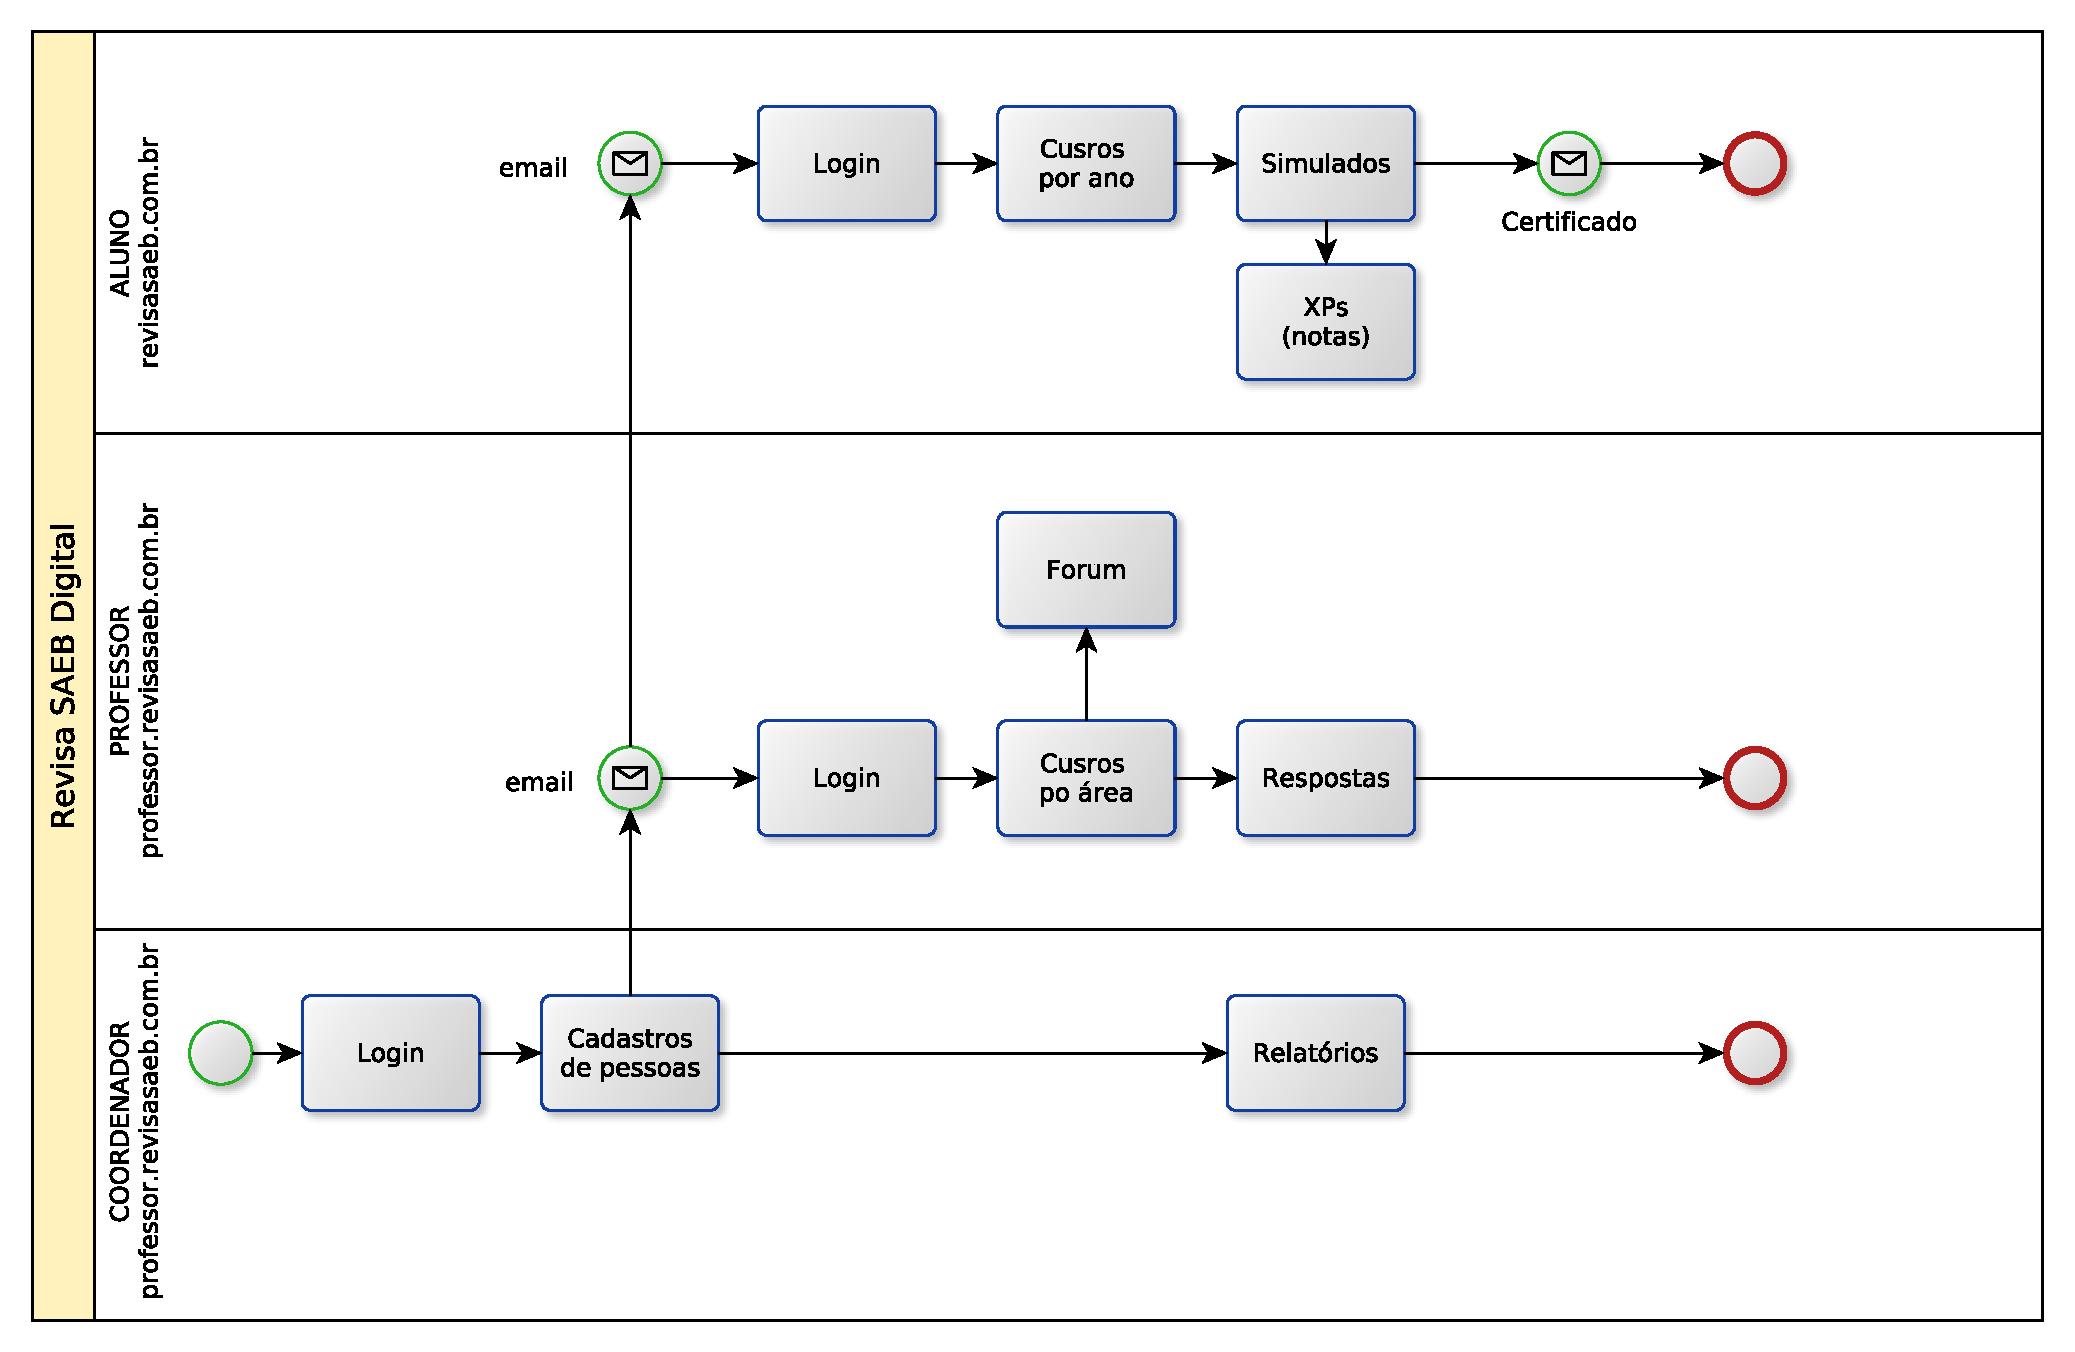
\includegraphics[width=\textwidth]{imgs/bpmn}
\caption{Estrutura da Plataforma por perfis de acesso}
\end{figure}

\end{itemize}

Para testes, entre no endereço \textbf{revisasaeb.com.br} com 
as credenciais \textbf{aluno-teste} e senha \textbf{minhacidade}. 


 

\chapter{Imagens do site}

\begin{figure}
\includegraphics[width=\textwidth]{imgs/front}
\caption{Home da Plataforma}
\end{figure}

% \begin{figure}
% \includegraphics[width=\textwidth]{imgs/login}
% \caption{Tela de login}
% \end{figure}


\begin{figure}
\includegraphics[width=\textwidth]{imgs/cursos}
\caption{Todos os cursos do aluno divididos por ano}
\end{figure}


\begin{figure}
\includegraphics[width=\textwidth]{imgs/jogo1}
\caption{Jogo sobre frações}
\end{figure}


\begin{figure}
\includegraphics[width=\textwidth]{imgs/jogo2}
\caption{Jogo sobre uso de dinheiro}
\end{figure}


\begin{figure}
\includegraphics[width=\textwidth]{imgs/video1}\bigskip

\includegraphics[width=\textwidth]{imgs/video-2}
\caption{Vídeos}
\end{figure}



\begin{figure}
\includegraphics[width=\textwidth]{imgs/progresso}
\caption{No perfil do aluno é possível ver o progresso de cada curso}
\end{figure}


\begin{figure}
\includegraphics[width=\textwidth]{imgs/relatorio}
\caption{Relatório detalhado por aluno}
\end{figure}


\begin{figure}
\includegraphics[width=.7\textwidth]{imgs/relatorio1}
\caption{Relatório para o coordenador ou professor}
\end{figure}

% André
% Explicar as seções, a relação com o material impresso, os quiz



